\documentclass{beamer}
\usepackage{mathtools}
\usepackage{xspace}
\usepackage{listings}
\usepackage{booktabs}
\usepackage{commath}

\DeclareMathOperator{\cond}{cond}
\let\arrowvec\vec
\renewcommand{\vec}[1]{\ensuremath{#1}}
\newcommand{\integral}[1]{\ensuremath{\int_{S^2} #1 \dif \Omega}}
\newcommand{\closure}[1]{\ensuremath{\mathcal{E}(#1)}}
\newcommand{\T}[1]{\ensuremath{#1^\textnormal{T}}}
\newcommand{\R}{\ensuremath{\mathbb{R}}\xspace}
\newcommand{\SN}{\ensuremath{\textnormal{S}_\textnormal{N}}\xspace}
\newcommand{\PN}{\ensuremath{\textnormal{P}_\textnormal{N}}\xspace}
\newcommand{\MN}{\ensuremath{\textnormal{M}_\textnormal{N}}\xspace}
\newcommand{\PPN}{\ensuremath{\textnormal{PP}_\textnormal{N}}\xspace}
\newcommand{\FPN}{\ensuremath{\textnormal{FP}_\textnormal{N}}\xspace}
\newcommand{\DN}{\ensuremath{\textnormal{D}_\textnormal{N}}\xspace}
\newcommand{\kinetic}{\texttt{kinetic}\xspace}
\newcommand{\moment}{\texttt{moment}\xspace}
\newcommand{\momopt}{\texttt{momopt}\xspace}

\usetheme{Madrid}
\beamertemplatenavigationsymbolsempty
\frenchspacing

\title{\texttt{closures-2d}}
\author{Tim Shaffer\thanks{Mentor: C. Kristopher Garrett}}

\begin{document}
    \frame{\titlepage}

    \begin{frame}{Goals}
        We are releasing software that tests angular approximations in kinetic transport simulations
        \begin{itemize}
            \item Based on code used for a previous publication~(Garrett and Hauck 2013)
            \item Open source so that others can use/collaborate
            \item Modular, making it easy to implement new features
            \item Implements \SN, \PN, \FPN, \MN, \PPN, \DN~(experimental)
        \end{itemize}

        \vfill

        \begin{columns}
            \column{0.4 \textwidth}
            \centering
            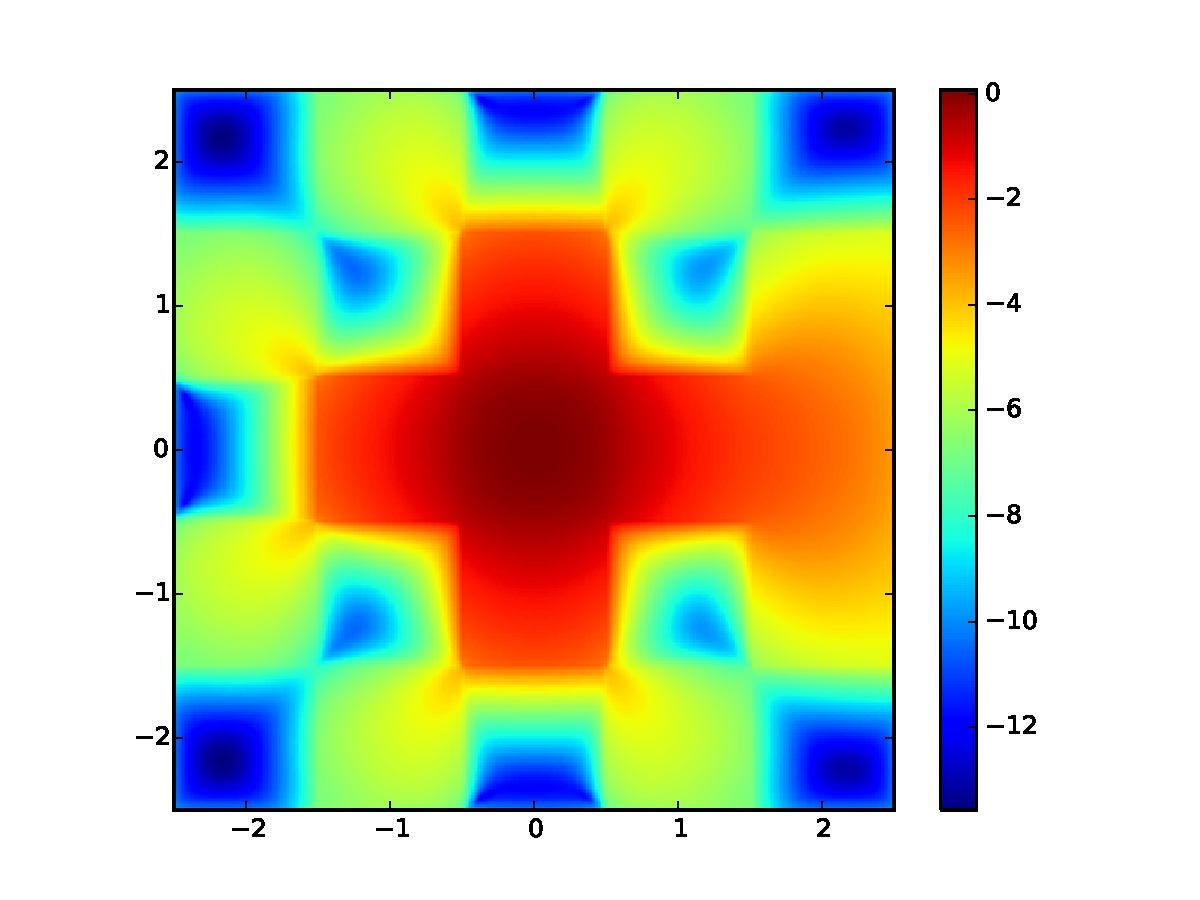
\includegraphics[width=\textwidth]{lattice.pdf}

            \PN Order 3

            \column{0.4 \textwidth}
            \centering
            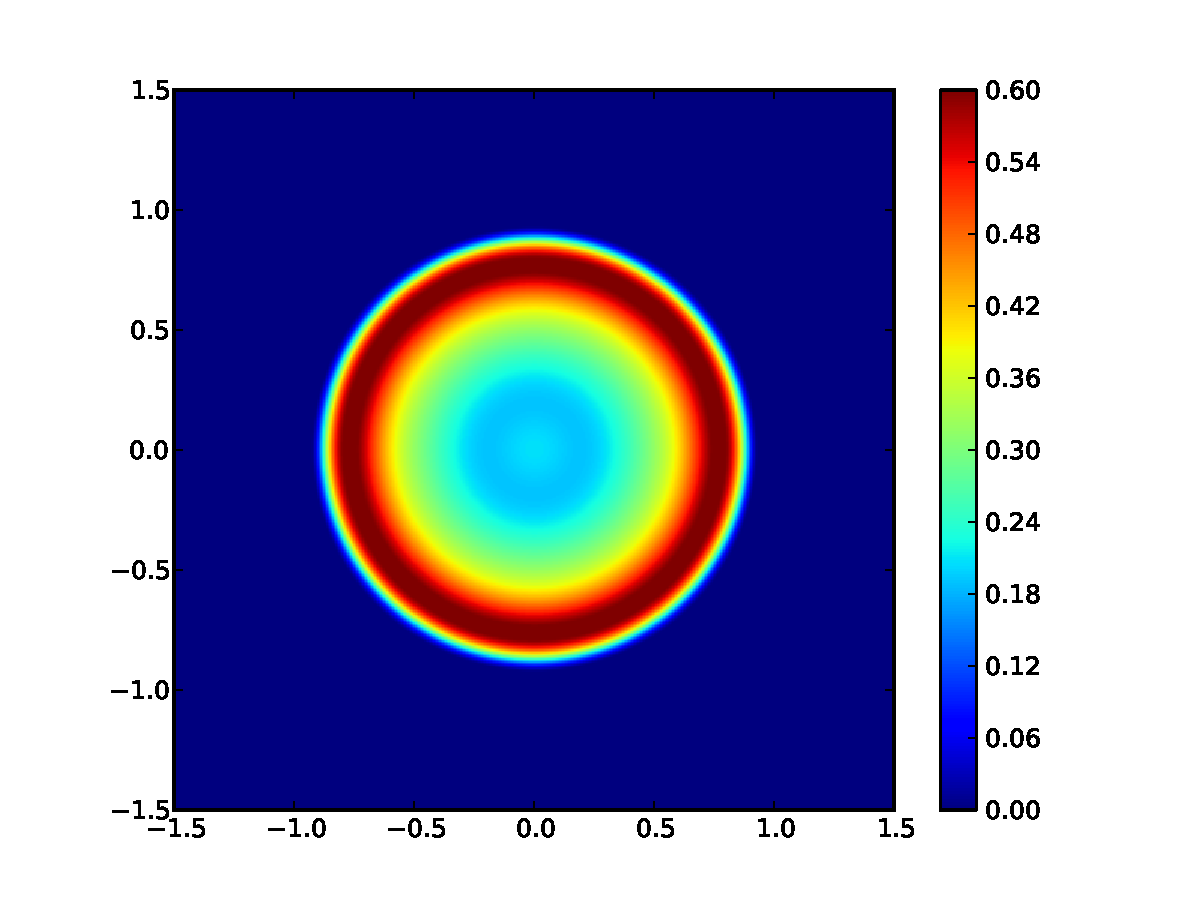
\includegraphics[width=\textwidth]{FP03-sspline-400-tune=20.pdf}

            \FPN(sspline) Order 3
        \end{columns}
    \end{frame}

    \begin{frame}{Improvements}
        Algorithmic changes:
        \begin{itemize}
            \item Added experimental Lebedev quadrature
            \item Removed $\gamma$ factor for ansatz correction in \texttt{momopt}
            \item Changed \texttt{momopt}'s regularization in case of bad condition number
        \end{itemize}

        \vfill

        Software-related improvements:
        \begin{itemize}
            \item Cross-platform build system
            \item Automated testing
            \item Better MPI communication
            \item Improved documentation
            \item Improved interface
            \item Bugfixes
            \item Profiling and optimization
        \end{itemize}
    \end{frame}

    \begin{frame}{Release}
        We are releasing this code as open source software.

        \vfill

        Now uses SCons, a Python-based build system, rather than Makefiles
        \begin{itemize}
            \item Cross platform
            \item Sets up library search paths
            \item Intelligent compilation
        \end{itemize}

        \vfill

        Depends on:
        \begin{columns}
            \column{0.25 \textwidth}
            \begin{itemize}
                \item GSL
                \item BLAS
                \item LAPACK
            \end{itemize}
            \column{0.4 \textwidth}
            \begin{itemize}
                \item OpenMP (optional)
                \item MPI (optional)
                \item PAPI (optional)
            \end{itemize}
        \end{columns}
    \end{frame}

    \begin{frame}{What Are Kinetic Equations?}
        \begin{columns}[t]
            \column{0.45 \textwidth}
            \begin{block}{Macroscopic}
                \begin{itemize}
                    \item $\rho(\vec{x},t)$ -- Density
                    \item $\vec{u}(\vec{x},t)$ -- Velocity
                    \item $E(\vec{x},t)$ -- Kinetic Energy
                \end{itemize}
                Discretize \vec{x}, $t$ into 100 values: 4GB memory requirement
            \end{block}
            \column{0.45 \textwidth}
            \begin{block}{Mesoscopic}
                \begin{itemize}
                    \item $f(\vec{x},\vec{v},t)$ -- Density with respect to space \emph{and velocity}
                \end{itemize}
                Discretize \vec{x}, \vec{v}, $t$ into 100 pieces: 800TB memory requirement
            \end{block}
        \end{columns}

        \vfill

        Macroscopic can be derived from mesoscopic
        \begin{itemize}
            \item $\rho(\vec{x},t) = \int_{\R^3} f \dif \vec{v}$
            \item $\vec{u}(\vec{x},t) = \frac{1}{\rho} \int_{\R^3} \vec{v}f \dif \vec{v}$
            \item $E(\vec{x},t) = \frac{1}{2} \int_{\R^3} \| \vec{v} - \vec{u} \|^2 \dif \vec{v}$
        \end{itemize}
    \end{frame}

    \begin{frame}{What Are Kinetic Equations?}
        First used for rarefied gas dynamics (e.g. high altitude gases where collisions do not dominate the physics)

        \[\partial_t f + \vec{v} \cdot \nabla_\vec{x} = C(f)\]
        where $\int C(f) \dif \vec{v} = 0$.

        \vfill

        Integrate against \vec{v} to get First Euler/Navier-Stokes equation
        \[\partial_t \rho + \nabla_{\vec{x}} \cdot (\rho \vec{u}) = 0\]

        \vfill

        Other areas:
        \begin{itemize}
            \item Radiation transport
            \item Plasma simulations
        \end{itemize}
    \end{frame}

    \begin{frame}{Kinetic Problem}
        \begin{block}{Unit Speed, Isotropic Scattering}
            \begin{equation*}
                \partial_t f + \Omega \cdot \nabla_\vec{x} = \frac{\sigma_s}{4\pi} \integral{f} - \sigma_t f
            \end{equation*}
            where $x \in \R^3$, $\Omega \in S^2$, and $\sigma_s$,$\sigma_t$ are the scattering and transmission cross sections.
        \end{block}

        \vfill

        \begin{columns}
            \column{0.33 \textwidth}
            \centering
            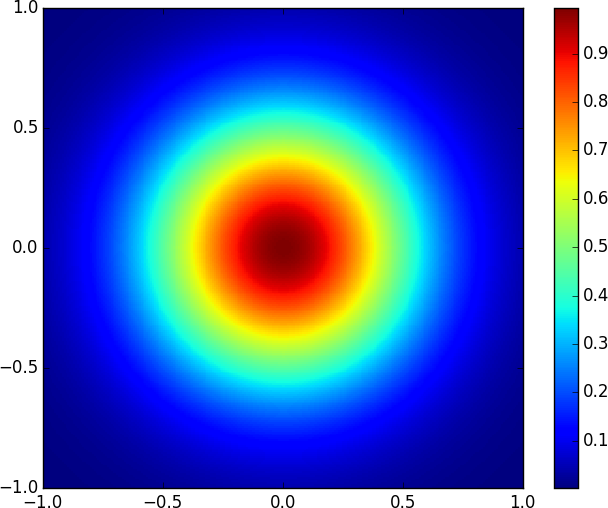
\includegraphics[width=\textwidth]{initcond_gaussian.png}

            \column{0.33 \textwidth}
            \centering
            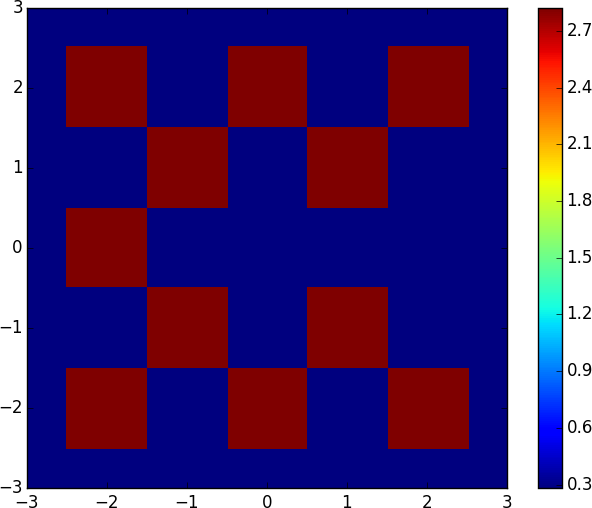
\includegraphics[width=\textwidth]{initcond_lattice-t.png}

            \column{0.33 \textwidth}
            \centering
            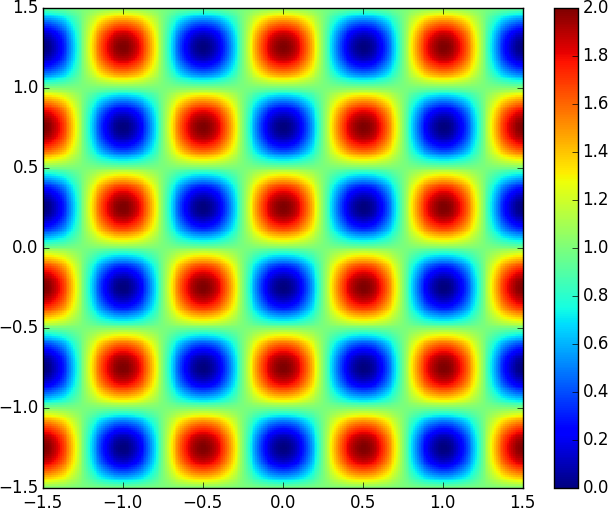
\includegraphics[width=\textwidth]{initcond_smooth.png}
        \end{columns}
        \begin{columns}
            \column{0.33 \textwidth}
            \centering
            Gaussian Initial Condition

            \column{0.33 \textwidth}
            \centering
            $\sigma_T$ for Lattice Initial Condition

            \column{0.33 \textwidth}
            \centering
            Smooth Initial Condition
        \end{columns}
    \end{frame}

    \begin{frame}{\kinetic}
        \begin{columns}
            \column{0.66 \textwidth}
            \begin{itemize}
                \item Implements \SN
                \item Easy to compute
                \item Permits negative densities
                \item Suffers from ray effects at low order
            \end{itemize}

            \column{0.33 \textwidth}
            \centering
            \includegraphics[width=\textwidth]{gaussian.pdf}

            Analytic Solution
        \end{columns}

        \vfill

        \begin{columns}
            \column{0.33 \textwidth}
            \centering
            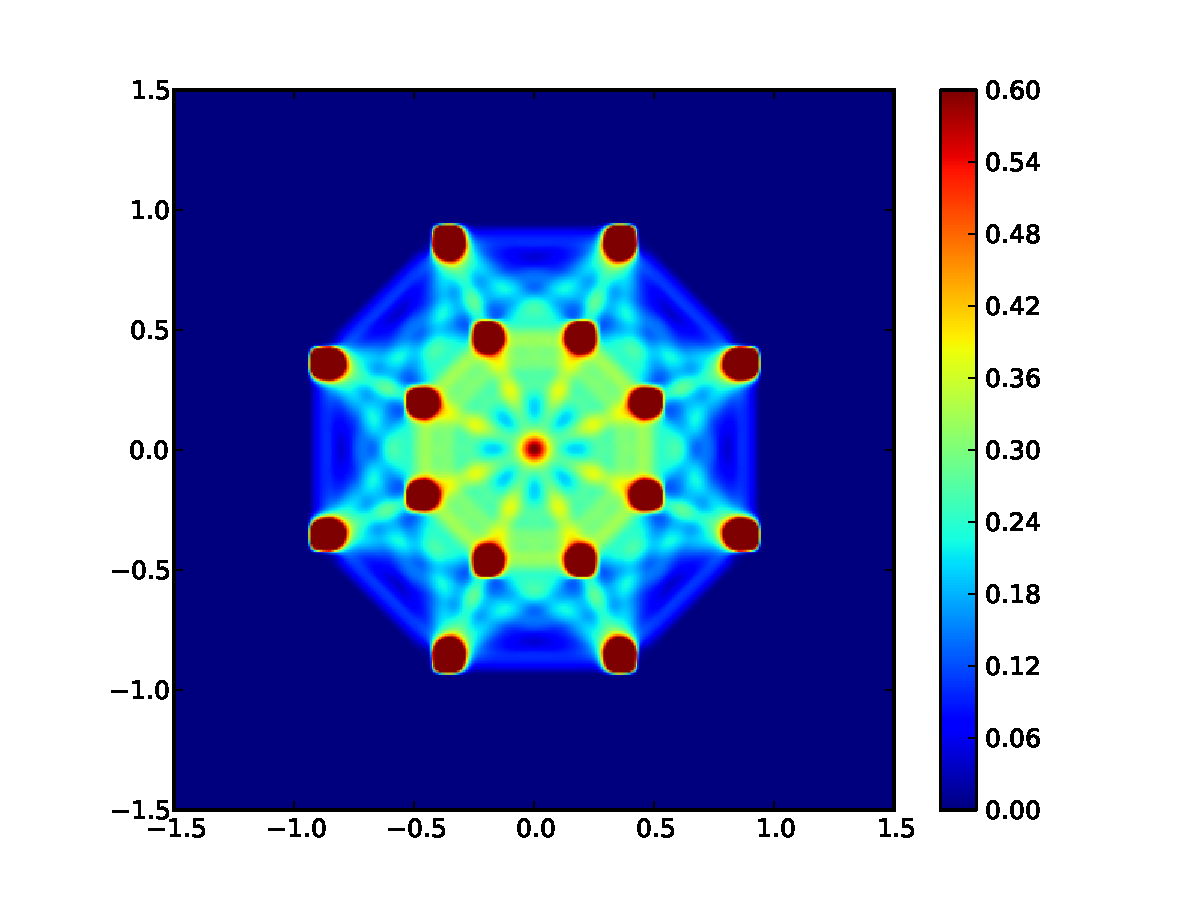
\includegraphics[width=\textwidth]{S04-400.pdf}

            \SN Order 4

            \column{0.33 \textwidth}
            \centering
            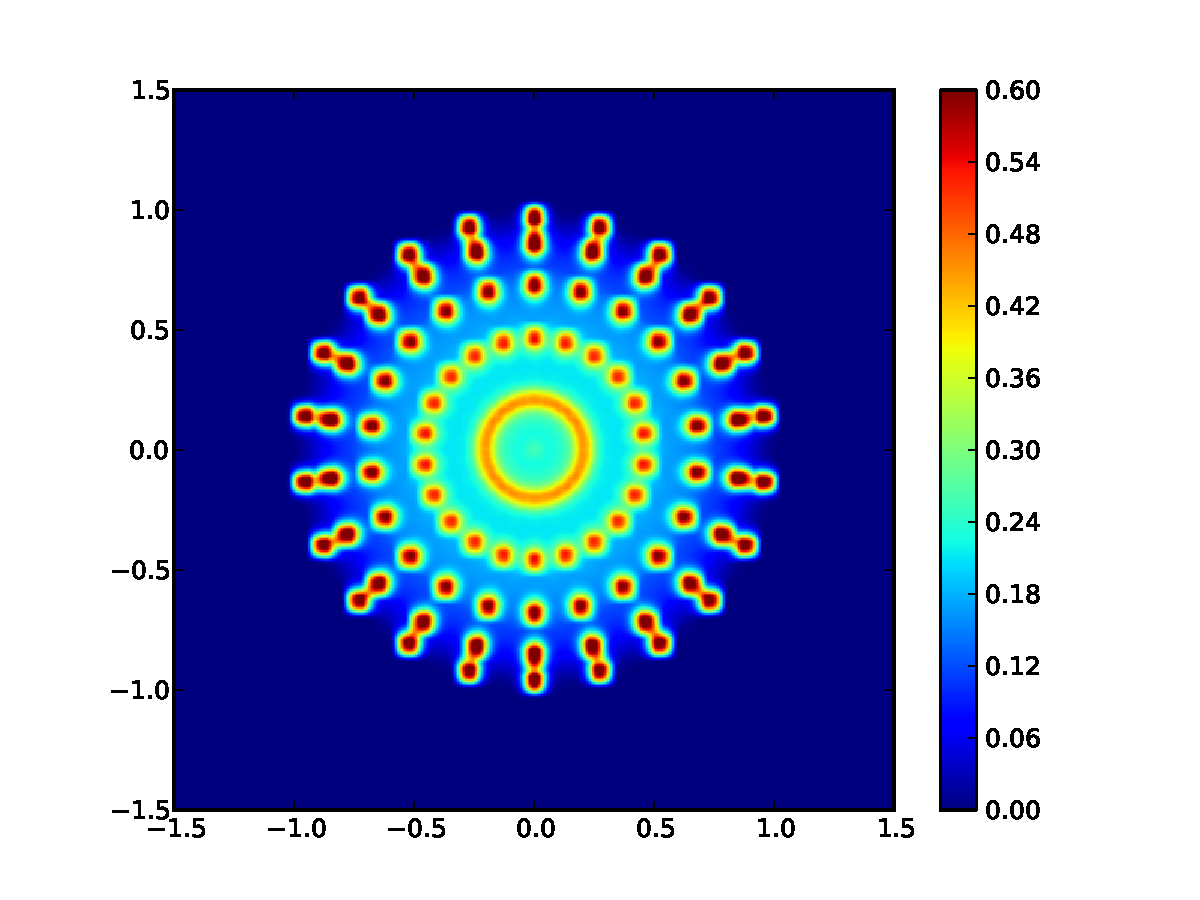
\includegraphics[width=\textwidth]{S11-400.pdf}

            \SN Order 11

            \column{0.33 \textwidth}
            \centering
            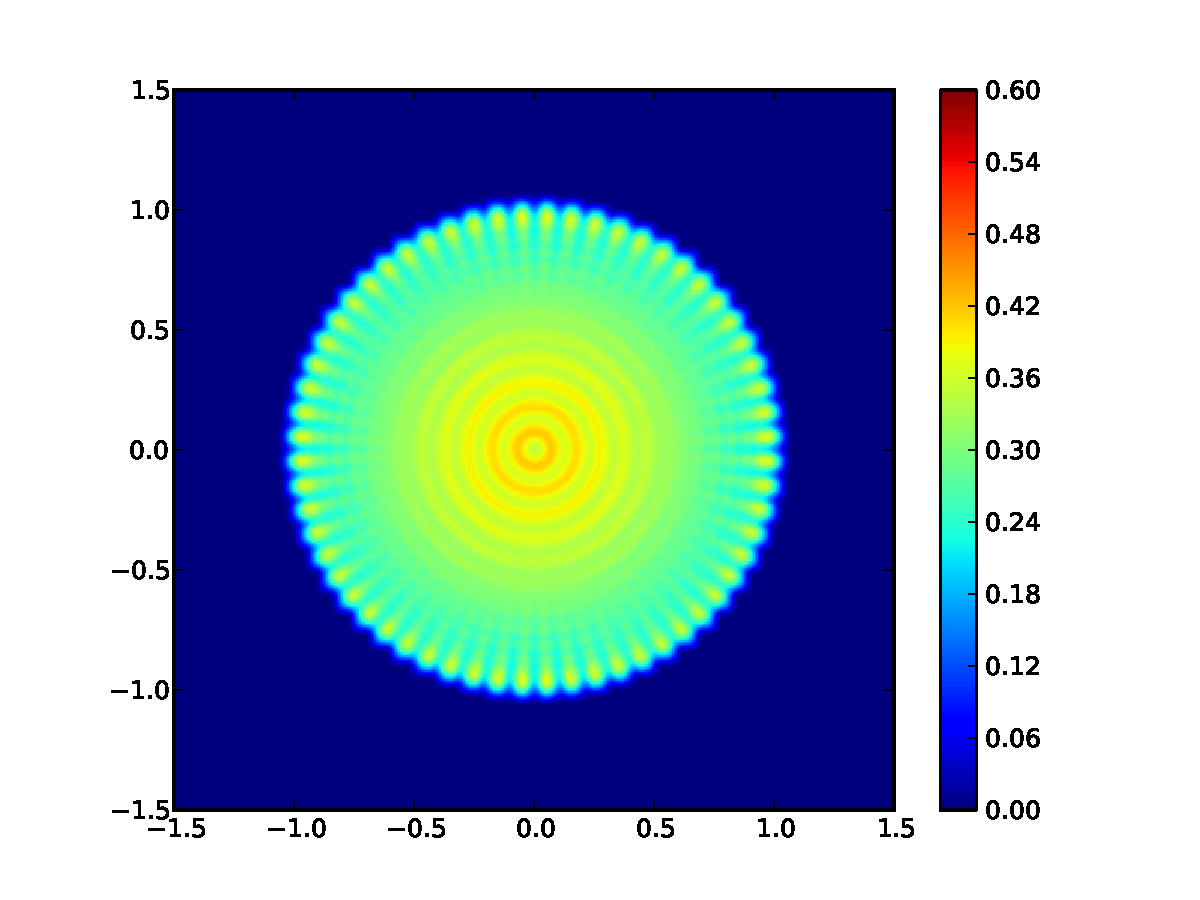
\includegraphics[width=\textwidth]{S30-400.pdf}

            \SN Order 30
        \end{columns}
    \end{frame}

    \begin{frame}{\moment}
        \begin{itemize}
            \item Implements \PN, \FPN
            \item Somewhat easy to compute
            \item Permits negative densities
            \item Suffers from oscillatory artifacts
            \item Filters can improve performance
        \end{itemize}

        \vfill

        \begin{columns}
            \column{0.5 \textwidth}
            \centering
            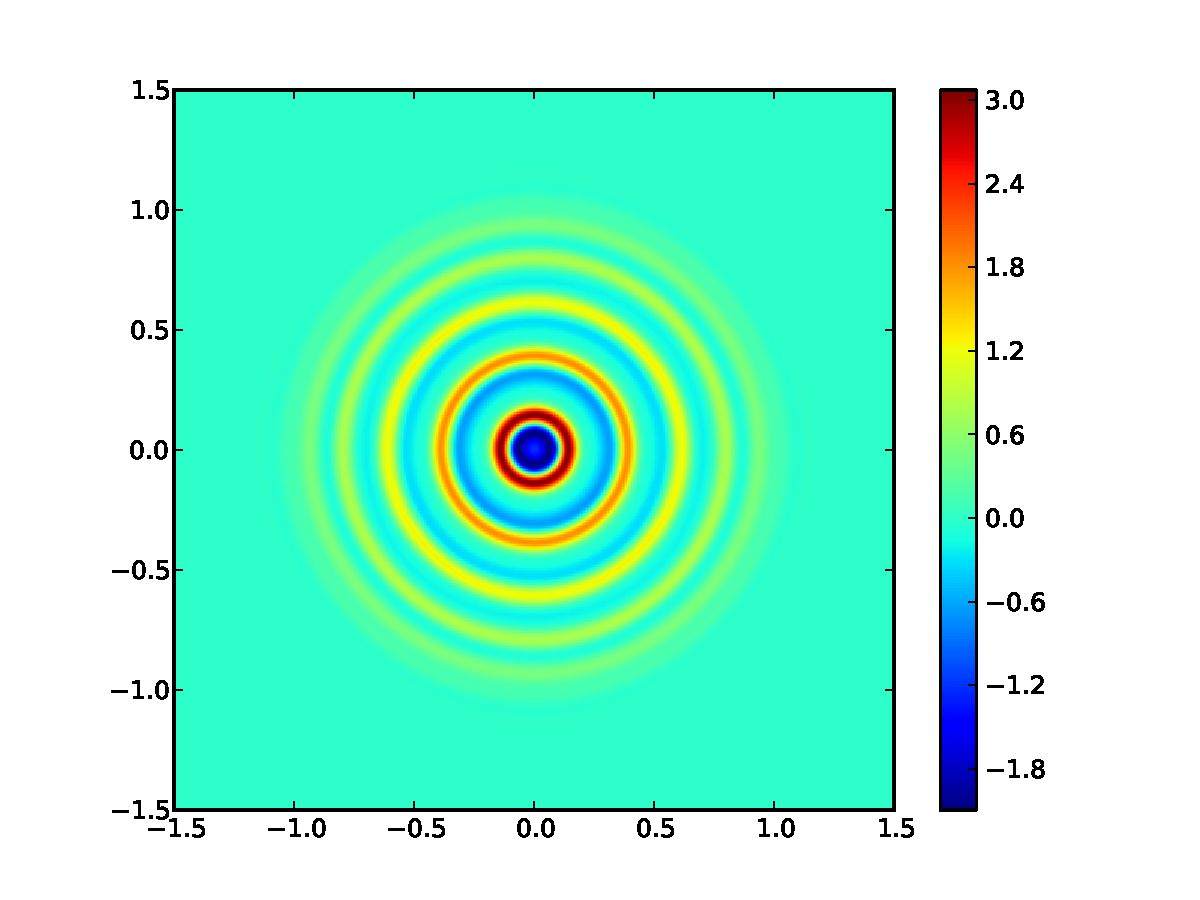
\includegraphics[width=\textwidth]{P11-400.pdf}

            \PN Order 11

            \column{0.5 \textwidth}
            \centering
            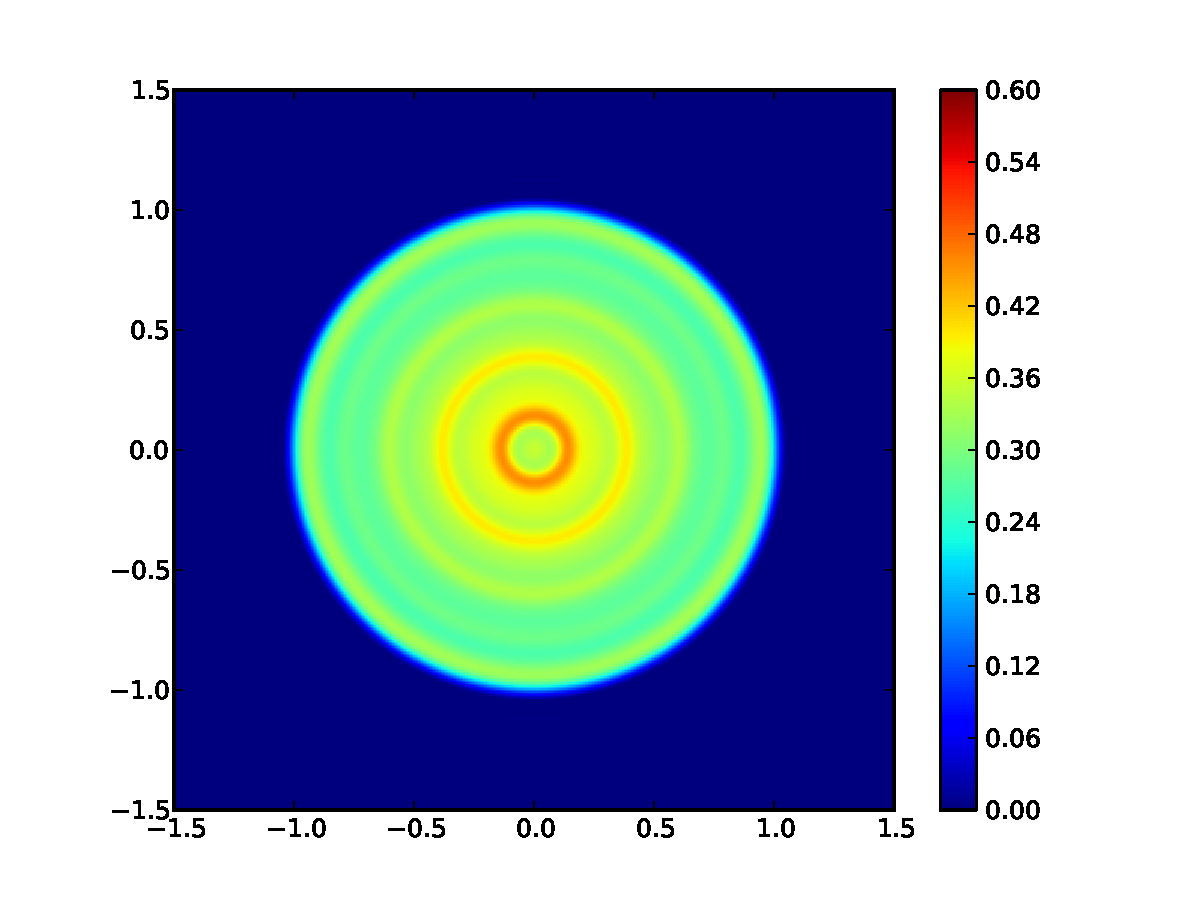
\includegraphics[width=\textwidth]{FP11-lanczos-400-tune=10.pdf}

            \FPN(Lanczos) Order 11
        \end{columns}
    \end{frame}

    \begin{frame}{\momopt}
        \begin{itemize}
            \item Implements \MN and \PPN
            \item Difficult to compute
            \item Ensures positivity
            \item Requires additional optimization procedure
        \end{itemize}

        \vfill

        \begin{columns}
            \column{0.5 \textwidth}
            \centering
            \includegraphics[width=\textwidth]{PP11-S30-400.pdf}

            \PPN Order 11

            \column{0.5 \textwidth}
            \centering
            \includegraphics[width=\textwidth]{M11-S30-400.pdf}

            \MN Order 11
        \end{columns}
    \end{frame}

    \begin{frame}[fragile=singleslide]{Testing}
        We implemented several automated tests for the software.
        The testing code is written in Python and integrated with the build system.

        \vfill

        The testing code carries out
        \begin{itemize}
            \item Regression tests -- compare output to reference data included with the software
            \item Mass Conservation tests -- check that total density remains the same
            \item Convergence tests -- measure the effect of decreasing the cell size on the precision of the output
        \end{itemize}

        \vfill

        \begin{block}{Convergence: \moment (\texttt{sspline})}
            \centering
            \begin{tabular}{ccc}
                \toprule
                Cell size       & Error     & Order \\
                \midrule
                $\Delta x / 1$ & 8.075049 & 1.954163 \\
                $\Delta x / 2$ & 2.083932 & 2.082828 \\
                $\Delta x / 4$ & 0.491915 & 2.340759 \\
                $\Delta x / 8$ & 0.097107 & ---      \\
                \bottomrule
            \end{tabular}
        \end{block}
    \end{frame}


    \begin{frame}{Performance}
        Added timing and profiling-related measurement capabilities

        \vfill

        Tested additional optimizations
        \begin{itemize}
            \item Spatial blocking (reduce scheduling overhead, cache misses)
            \item CPU pinning (ccNUMA)
            \item Memory alignment
        \end{itemize}
    \end{frame}

    \begin{frame}[fragile=singleslide]{Caching Example: Matrix Multiplication}
        \begin{lstlisting}[language=C]
for(int i = 0; i < N; i++) {
for(int j = 0; j < N; j++) {
for(int k = 0; k < N; k++) {
    result[i][j] += left[i][k] * right[k][j]
}}}
        \end{lstlisting}
    \end{frame}

    \begin{frame}[fragile=singleslide]{Caching Example: Matrix Multiplication}
        \begin{lstlisting}[language=C]
for(int i = 0; i < N; i++) {
for(int k = 0; k < N; k++) {
for(int j = 0; j < N; j++) {
    result[i][j] += left[i][k] * right[k][j]
}}}
        \end{lstlisting}
    \end{frame}

    \begin{frame}{Caching Example: Matrix Multiplication}
        \begin{center}
            \begin{tabular}{cc}
                \toprule
                Loop order & Time \\
                \midrule
                ijk & 8.139175 \\
                ikj & 5.316213 \\
                jik & 6.160773 \\
                jki & 19.494467 \\
                kij & 5.406215 \\
                kji & 19.666042 \\
                \bottomrule
            \end{tabular}
        \end{center}

        \vfill

        \alert{Factor of 4 difference}
    \end{frame}

    \begin{frame}{Blocking}
        Cache utilization:
        \begin{itemize}
            \item Using a simple loop: move over each row and column, fetching values from main memory on \emph{every iteration}
            \item Using a block-oriented loop: compute one section, fetching most nearby values from a CPU cache
        \end{itemize}

        \vfill

        OpenMP Scheduling:
        \begin{itemize}
            \item Using a simple loop: dispatch each cell to a (possibly different) core
            \item Using a block-oriented loop: dispatch an entire block to core, improving cache utilization and reducing scheduling overhead
        \end{itemize}
    \end{frame}

    \begin{frame}{Quadratures}
        Currently uses Chebyshev-Legendre quadrature.
        \begin{itemize}
            \item Product quadrature on the sphere \[\int_{S^2} \cdot \dif \Omega = \int_{\mu=-1}^1 \int_{\phi=0}^{2\pi} \cdot \dif \phi \dif \mu\]
            \item $n$ Gauss-Legendre points on $\mu$
            \item $2n$ equally spaced points on $\phi$
            \item Exactly integrates to degree $2n - 1$ moments
            \item Easily optimized for symmetry
        \end{itemize}
    \end{frame}

    \begin{frame}{Quadratures}
        Added (experimental) Lebedev quadrature
        \begin{itemize}
            \item Constructed based on octahedral symmetry group
            \item Asymptotically optimal with respect to number of points

            (2/3 that of Chebyshev-Legendre)
            \item Structure does not lend itself to symmetry optimizations
            \item \alert{Negative weights break positivity}
        \end{itemize}
    \end{frame}

    \begin{frame}{Optimization Problem}
        \momopt uses nonlinear spectral methods, so updates entail solving an optimiztion problem for a given constant vector \vec{u} and moments $\vec{m}(\Omega)$.
        \begin{equation*}
            \min_{\vec{\alpha}} \integral{\exp(\T{\vec{\alpha}} \vec{m})} - \T{\vec{\alpha}} \vec{u}
        \end{equation*}

        \vfill

        To use a Newton solver, we need
        \begin{align*}
            \textnormal{Objective funtion } F(\vec{\alpha}) &= \integral{\exp(\T{\vec{\alpha} \vec{m}})} - \T{\vec{\alpha}} \vec{u} \\
            \textnormal{Gradient } g(\vec{\alpha}) &= \integral{\vec{m} \exp(\vec{\T{\alpha}} \vec{m})} - \vec{u} \\
            \textnormal{Hessian } H(\vec{\alpha}) &= \integral{\vec{m} \T{\vec{u}} \exp(\T{\vec{\alpha}} \vec{m})}
        \end{align*}

        \vfill

        Now the estimated $\vec{\alpha}_{i+1} = \vec{\alpha}_i + t\vec{d}$ where $\vec{d} = -H(\vec{\alpha})^{-1}g(\vec{\alpha})$.
    \end{frame}

    \begin{frame}{$\gamma$ factor}
        In \momopt's optimization steps, we compute an approximate \vec{\alpha} for a given \vec{u} such that $\vec{u} \approx \integral{\vec{m} \exp (\T{\vec{\alpha}} \vec{m})}$.
        \begin{itemize}
            \item Needed to estimate error and try to correct via $\gamma = \frac{\exp(\T{\bar{\vec{\alpha}}} \vec{m})}{\exp(\T{\hat{\vec{\alpha}}} \vec{m})}$.

                Here, the numerator of $\gamma$ is our approximation, and the denominatior is exact.
            \item Required fine mesh and low tolerance on optimization to prevent non-realizability.
        \end{itemize}

        \vfill

        Instead, compute $\hat{\vec{u}}$ such that $\hat{\vec{u}} = \integral{\vec{m} \exp(\T{\hat{\vec{\alpha}}} \vec{m})}$
        \begin{itemize}
            \item Adjust scaling to conserve mass
            \item \alert{Exact equality ensures positivity}
        \end{itemize}
    \end{frame}

    \begin{frame}{Fixed regularization}
        If $\cond(H(\vec{\alpha}))$ is too large
        \begin{itemize}
            \item $H(\vec{\alpha})$ is difficult to invert
            \item Can't find the direction $\vec{d} = -H(\vec{\alpha})^{-1}g(\vec{\alpha})$
        \end{itemize}

        \vfill

        Need to adjust the problem to make it more tractable
        \begin{itemize}
            \item Set isotropic initial guess

                $\vec{\alpha} = (2\sqrt{\pi} \log \frac{1}{2\sqrt{\pi}}, 0, 0, \dots, 0)$ for \MN,

                $\vec{\alpha} = (1 - 4\pi\delta, 0, 0, \dots, 0)$ for \PPN, where $\delta$ is a parameter of \PPN
            \item For $i = 2,\dots$, multiply each $u_i$ by $1 - r$, where $r$ is a regularization constant with $0 < r < 1$
        \end{itemize}
    \end{frame}

    \begin{frame}{Source Code}
        The source code is available on Github

        \url{https://github.com/ckrisgarrett/closures-2d}

        \vfill

        \begin{columns}
            \column{0.33 \textwidth}
            
\includegraphics[width=\textwidth]{DOESClogo.png}
            \column{0.33 \textwidth}
            
\includegraphics[width=\textwidth]{ORISElogo.png}
        \end{columns}
    \end{frame}
\end{document}
